%----------------------------------------------------------------------------
%----------------------------------------------------------------------------
The experiment requires three properly conditioned pulses, all incident upon the same spatial region, sequenced in a specific temporal order. A single Nd:YAG pulsed dye laser is used to simultaneously pump three dye lasers; thus the relative delay between each dye laser is fixed. We will obtain arbitrary control of the pulse sequence by delaying two pulses with respect to the third. By manipulating the beam line design, we can force all three pulses to be temporally coincident while the delay lines are in their middle positions. In this way each of the two delayed pulses can be retarded or advanced by 4 ns with respect to the un-delayed pulse. We can even swap dye cells between dye lasers for complete control of the color order in the pulse sequence.

Once the pulses are properly delayed and ordered, they are aligned in a ``beam mixer'' so that their optical axes are collinear. The final output of the laser system is a three color transform limited pulse sequence with user specified color triple, amplitude triple, and relative delay of the pulses within the sequence. We use a 50/50 beam splitter as the beam mixer. Since we do not yet know the optimal color sequence, in the initial stages of this experiment, we will use broadband 50/50 beam splitters as we explore different color sets. Once the optimal color sequence is set, then more efficient optics could be specified if required. See figure \ref{block_three_dye}.
%----------------------------------------------------------------------------
% block_three_dye.tex
% by Troy Hix, May 2005
%----------------------------------------------------------------------------
\begin{figure}
\center
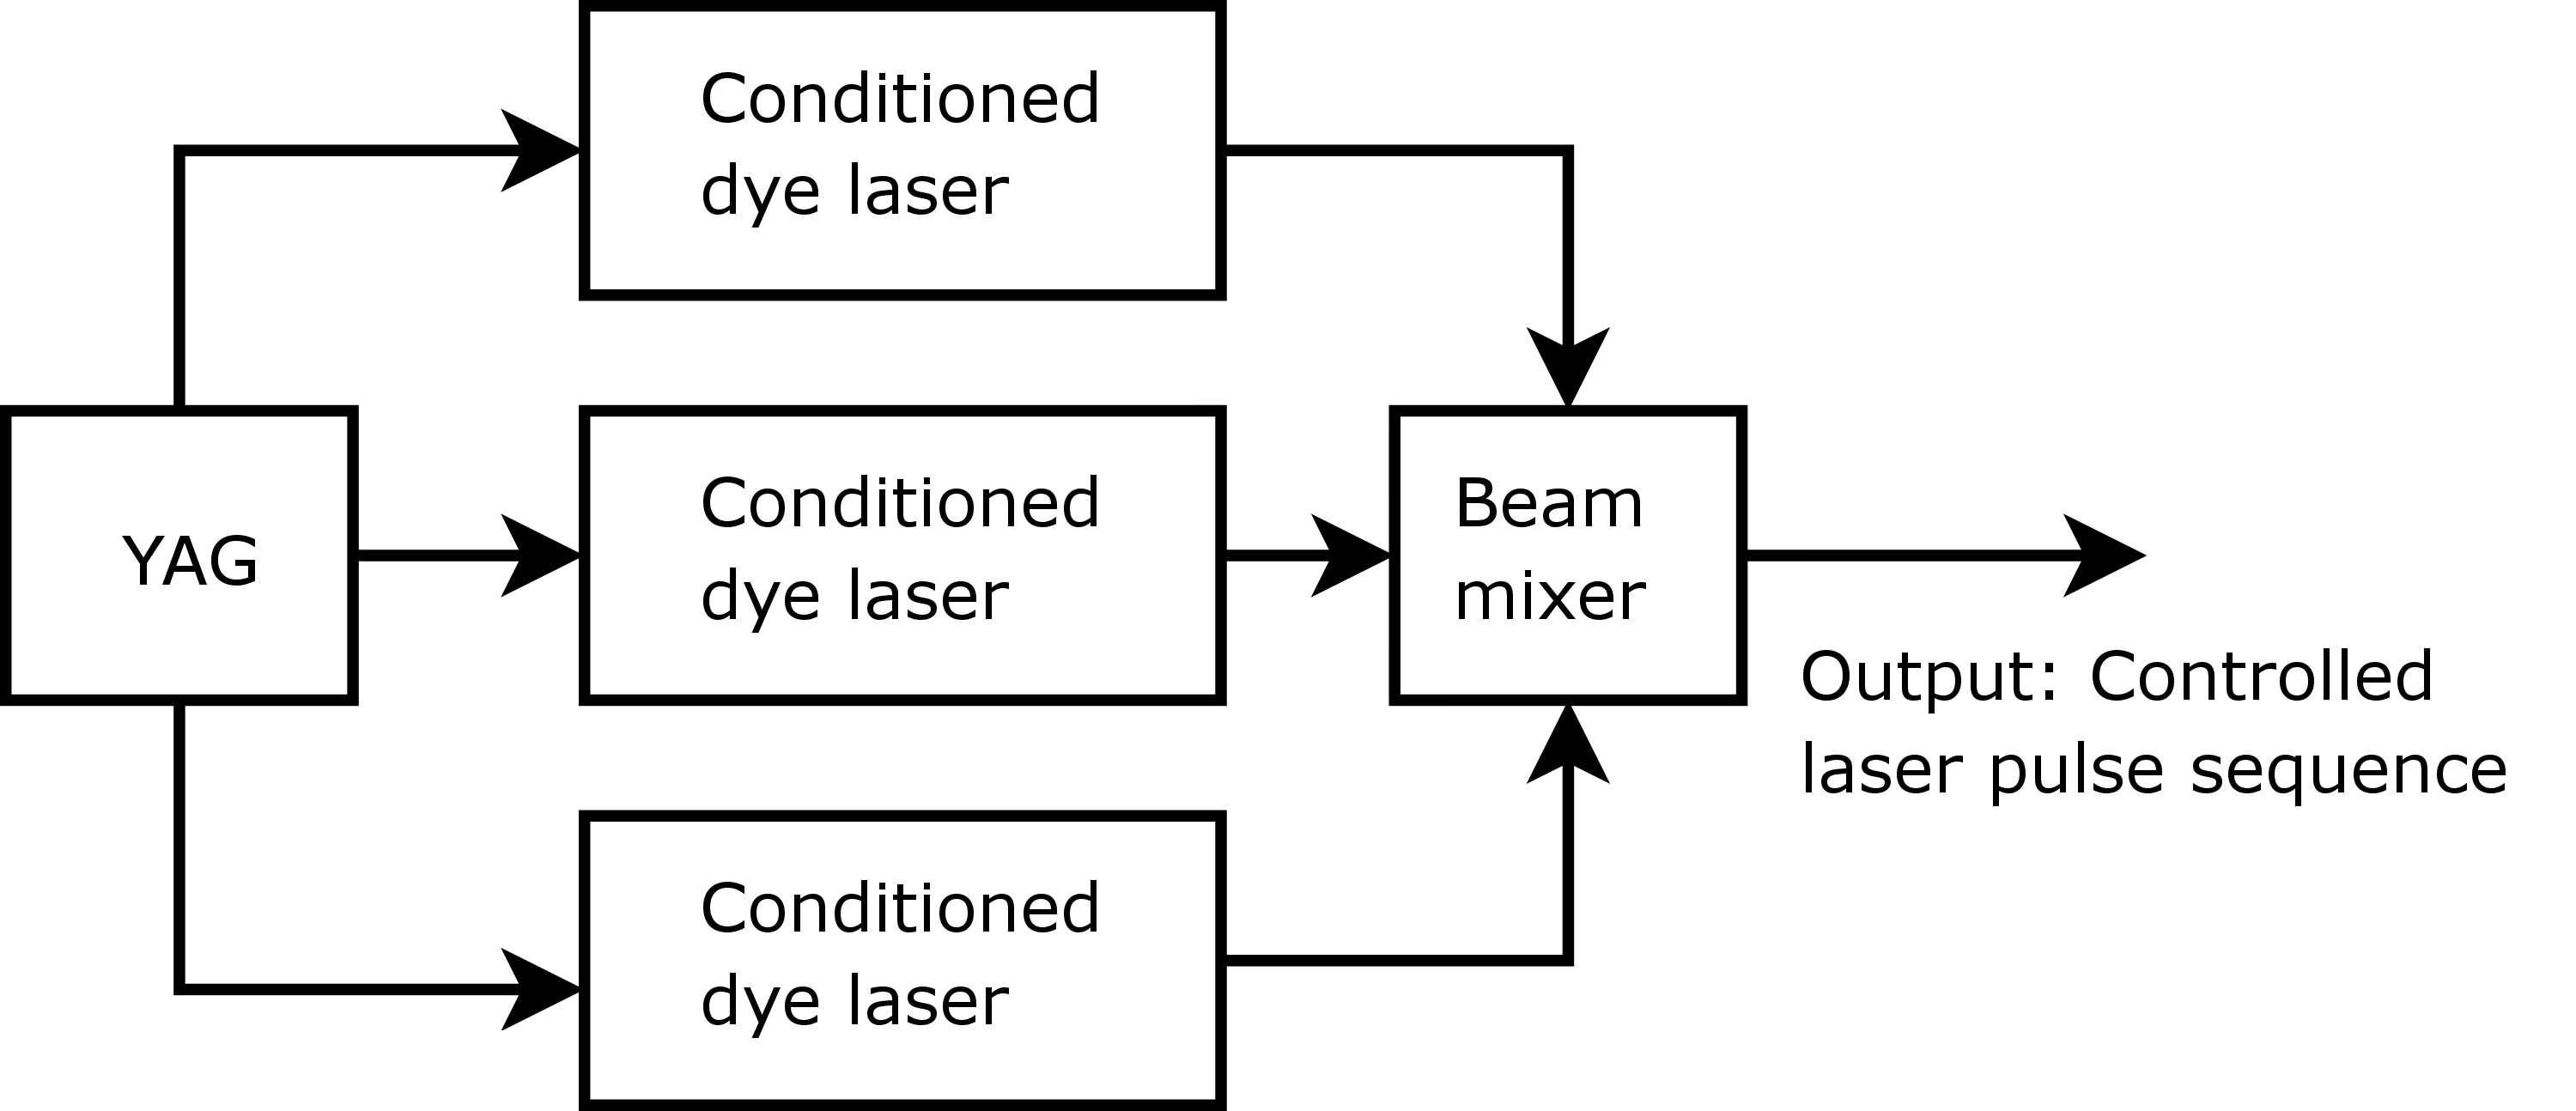
\includegraphics[width=4.00in]
{block_three_dye/block_three_dye.png}\\
\caption{Three conditioned and synchronized dye lasers block diagram}
\label{block_three_dye}
\end{figure} 
%----------------------------------------------------------------------------
%----------------------------------------------------------------------------
%----------------------------------------------------------------------------



%----------------------------------------------------------------------------
%----------------------------------------------------------------------------
%----------------------------------------------------------------------------
%----------------------------------------------------------------------------
%----------------------------------------------------------------------------
